\documentclass{article}
\usepackage[T1]{fontenc}
\usepackage{lmodern}
\usepackage{graphicx}
\usepackage{amsmath,amssymb}
\usepackage[a4paper,margin=2cm]{geometry}
\usepackage[absolute,overlay]{textpos}
\setlength{\TPHorizModule}{1mm}
\setlength{\TPVertModule}{1mm}
\usepackage[indonesian]{babel}
\usepackage{hyperref}
\setlength{\emergencystretch}{2em}
% unit: Halaman 32

\begin{document}

% === Halaman 32 (llm) ===

\vspace{121.77mm}

Sumber: Introduction to Practical Cryptography, Lecture 3 Block Ciphers

% deskripsi: Diagram alur proses enkripsi block cipher yang menunjukkan tahapan dari Plaintext menjadi Ciphertext, mencakup IP, 32 rounds (whitening, S-Box, Linear Transformation), IP-1, dan keterangan mengenai kunci 256 bit serta operasi bitwise.
% bbox normalisasi: [0.1500, 0.4700, 0.7700, 0.8800]
\begin{textblock*}{130.20mm}(31.50mm,139.59mm)
\noindent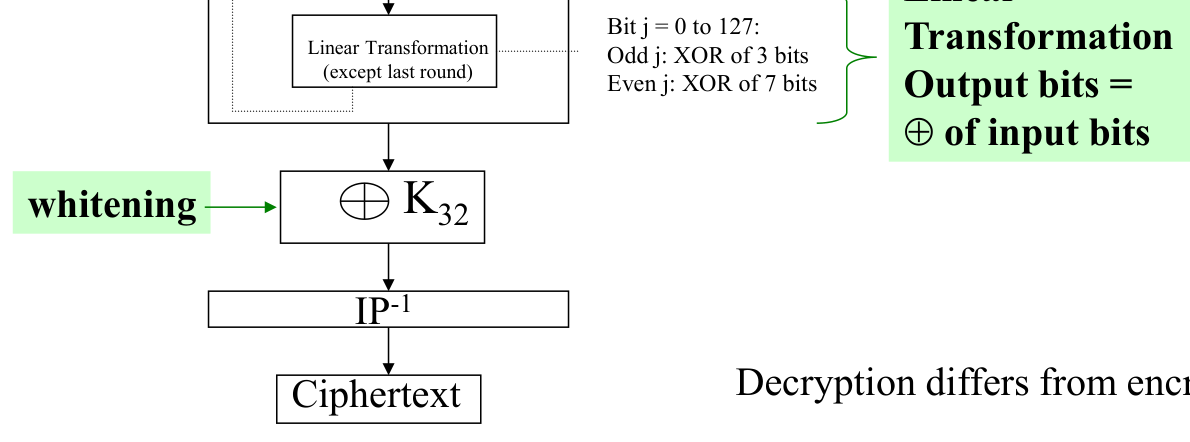
\includegraphics[width=130.20mm,height=121.77mm]{../../images/llm/page_032_img_01.png}%
\end{textblock*}

\end{document}
